
\chapter{Quantum Circuits}





\section{Composite Systems}

\begin{example}
For one system with state $\frac{1}{\sqrt{2}} \ket{0} + \frac{1}{\sqrt{2}} \ket{1}$
and second system with state $\frac{1}{\sqrt{2}} \ket{0} + \frac{\sqrt{3}}{2} \ket{1}$ 
find the state of the \textit{composite system}.
\end{example}

\frameans{}{
$
\frac{1}{2\sqrt{2}} \ket{00} + 
\frac{\sqrt{3}}{2\sqrt{2}} \ket{01} + 
\frac{1}{2\sqrt{2}} \ket{10} + 
\frac{\sqrt{3}}{2\sqrt{2}} \ket{11}
$ 
}

\begin{example}
Prove that the following two-qubit system \textit{cannot be factorised}
into two qubits. 
$$\ket{\psi} = \frac{1}{\sqrt{2}} \ket{00} + \frac{1}{\sqrt{2}} \ket{11}$$
\end{example}

\frmrule

\[ \begin{array}{lll}
\ket{\psi} = \frac{1}{\sqrt{2}} \ket{00} + \frac{1}{\sqrt{2}} \ket{11} 
& = & (\alpha_0 \ket{0} + \alpha_1 \ket{1})(\beta_0 \ket{0} + \beta_1 \ket{1}) \\
& = & \alpha_0 \beta_0 \ket{00} + 
\alpha_0 \beta_1 \ket{01} + 
\alpha_1 \beta_0 \ket{10} + 
\alpha_1 \beta_1 \ket{11} \\
\end{array}\] 

Comparing coefficients we have the following: \\
$\alpha_0 \beta_0 = \frac{1}{\sqrt{2}}$,
$\alpha_0 \beta_1 = 0$,
$\alpha_1 \beta_0 = 0$ and
$\alpha_1 \beta_1 = \frac{1}{\sqrt{2}}$.

If we multiply eqn1 and eqn4 we get $\alpha_0 \alpha_1 \beta_0 \beta_1 = \frac{1}{2}$.
If we multiply eqn2 and eqn3 we get $\alpha_0 \alpha_1 \beta_0 \beta_1 = 0$.
And yet, $0 \neq \frac{1}{2}$. We have a contradiction and so the system has no solution. 



\section{Entangled Systems}



\section{Bell States}


Bell states are \textit{rotationally invariant}.
Given $\ket{\psi} = \frac{1}{\sqrt{2}} [\ket{uu} + \ket{u^{\perp}u^{\perp}}]$ 
and a rotation of the bit basis:
$\ket{u} = a\ket{0} + b\ket{1}$ with $\ket{u^{\perp}} = -b\ket{0} + a\ket{1}$




\[ \begin{array}{ll}
\ket{\psi}
& =
\frac{1}{\sqrt{2}} [\ket{uu} + \ket{u^{\perp}u^{\perp}}] \\
& =
\frac{1}{\sqrt{2}} [(a\ket{0} + b\ket{1})(a\ket{0} + b\ket{1}) 
+ (-b\ket{0} + a\ket{1})(-b\ket{0} + a\ket{1})]  \\ 
& =
\frac{1}{\sqrt{2}} [(a^2 + b^2)\ket{00} + (a^2 + b^2)\ket{11} \\ 
& =
\frac{1}{\sqrt{2}} [\ket{00} + \ket{11} \\ 
\end{array}\] 

\frmrule

The previous bell state is only rotationlly invariant for real valued rotations. 
It is not invariant for complex rotations. However the bell state, 
psi-minus, $\ket{\psi^{-}} = \frac{1}{\sqrt{2}} [\ket{01} - \ket{10}]$
is invariant under all complex rotations.

\begin{example}
Prove that the bell state $\ket{\psi^{-}}$ is invariant under all complex rotations.
\end{example}


\section{Introducing Quantum Circuits}



\begin{figure}
  \centerline{
    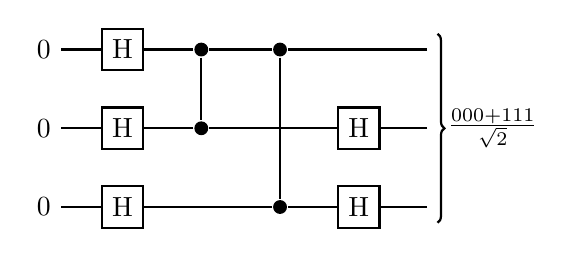
\begin{tikzpicture}[thick]
    %
    % `operator' will only be used by Hadamard (H) gates here.
    % `phase' is used for controlled phase gates (dots).
    \tikzstyle{operator} = [draw,fill=white,minimum size=1.5em] 
    \tikzstyle{phase} = [fill,shape=circle,minimum size=5pt,inner sep=0pt]
    \tikzstyle{surround} = [fill=black!10,drop shadow,draw=black]
    %
    % Qubits
    \node at (0,0) (q1) {\ket{0}};
    \node at (0,-1) (q2) {\ket{0}};
    \node at (0,-2) (q3) {\ket{0}};
    %
    % Column 1
    \node[operator] (op11) at (1,0) {H} edge [-] (q1);
    \node[operator] (op21) at (1,-1) {H} edge [-] (q2);
    \node[operator] (op31) at (1,-2) {H} edge [-] (q3);
    %
    % Column 3
    \node[phase] (phase11) at (2,0) {} edge [-] (op11);
    \node[phase] (phase12) at (2,-1) {} edge [-] (op21);
    \draw[-] (phase11) -- (phase12);
    %
    % Column 4
    \node[phase] (phase21) at (3,0) {} edge [-] (phase11);
    \node[phase] (phase23) at (3,-2) {} edge [-] (op31);
    \draw[-] (phase21) -- (phase23);
    %
    % Column 5
    \node[operator] (op24) at (4,-1) {H} edge [-] (phase12);
    \node[operator] (op34) at (4,-2) {H} edge [-] (phase23);
    %
    % Column 6
    \node (end1) at (5,0) {} edge [-] (phase21);
    \node (end2) at (5,-1) {} edge [-] (op24);
    \node (end3) at (5,-2) {} edge [-] (op34);
    %
    % Bracket
    \draw[decorate,decoration={brace},thick] (5,0.2) to
    node[midway,right] (bracket) {$\frac{\ket{000}+\ket{111}}{\sqrt{2}}$}
    (5,-2.2);
    \end{tikzpicture}
  }
  \caption{
    A quantum circuit for producing a GHZ state using
    Hadamard gates and controlled phase gates.
  }
\end{figure}